\documentclass[a4paper,11pt]{article}
\usepackage{setspace}
\onehalfspacing
  
\usepackage{caption}
\usepackage{titlesec}
\usepackage{graphicx}
\usepackage{listings}
\usepackage{xcolor}
\usepackage{fancyhdr}
\usepackage[a4paper,margin=1in]{geometry}
\usepackage{mdframed} %nice frames

\definecolor{light-gray}{gray}{0.95} %the shade of grey that stack exchange uses

\renewcommand{\thispagestyle}[1]{} % do nothing

\lstset{
  language=Python,
  aboveskip=3mm,
  belowskip=3mm,
  showstringspaces=true,
  columns=flexible,
  basicstyle={\small\ttfamily},
  numbers=none,
  numberstyle=\tiny\color{gray},
  keywordstyle=\color{blue},
  commentstyle=\color{red},
  breaklines=true,
  breakatwhitespace=true,
  tabsize=2
}

\graphicspath{ {./images/} }
\titlespacing{\section}{0pc}{1pc}{1pc}
 
\pagestyle{fancy}
\fancyhf{}
\rhead{Assignment 5}
\lhead{Internet Traffic Analysis using Wireshark}
\rfoot{Page \thepage}

 
\begin{document}
\title{\vspace{-1.0cm}\textbf{Internet Traffic Analysis using Wireshark}}
\author{
  \textbf{Tan Wei Xuan (49003140)}\\
  \texttt{tanweixuan@postech.ac.kr}
}
\date{\today}
\maketitle

\section{Project Overview}
\textit{\textbf{Wireshark 3.0.1}} is used to analyze the network traffic captured over a specified period of time.

\section{Traffic Analysis using Wireshark}
Analysis is done on the captured network traffic within the provided tracefile. Network Traffic is captured for a period of \textbf{59.088} seconds.

\subsection{Total Number of Packets and Bytes}
\begin{figure}[h!]
	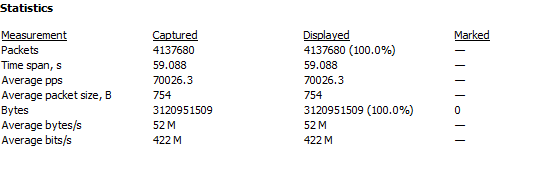
\includegraphics{TtlNoPacketsBytes}
	\caption{\textit{Capture Statistics (Statistics $\rightarrow$ Capture File Properties)}}
\end{figure}
The total number of packets being captured between a \textbf{59 second period} is \textbf{4137680}. The total number of Bytes between captured is \textbf{3120951509}. This information can be obtained thorugh \textit{Stastics $\rightarrow$ Capture File Properties}.

\subsection{Time Difference between First and Last Packet }
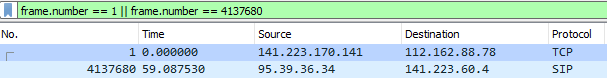
\includegraphics{TimeDiff}
\newline
\newline
We know that the total number of packets being captured is \textbf{4137680}. As such, the first frame be captured will be \textbf{1} and the last frame being captured will be \textbf{4137680}. We can filter out these two frames by applying the filter, \textit{\textbf{(frame.number $==$ 1) $||$ (frame.number $==$ 4137680)}}. From the filtered results, we can see that the first packet is being transmitted at \textbf{0.0} seconds while the last packet is being transmitted at \textbf{59.087530} seconds. As such, the \textbf{time difference} between the \textbf{first} and \textbf{last} packet is \textbf{59.087530 seconds}

\subsection{The number of packet and total bytes of TCP, UDP and ICMP traffic }
\begin{figure}[h!]
	\includegraphics[width = 16cm]{Traffic}
	\caption{\textit{TCP,UDP and ICMP Proticol Hierarchy (Statistics $\rightarrow$ Protocol Hierarchy)}}
\end{figure}
The entirety of the network traffic is being transmitted through \textbf{IPv4} as it takes up \textbf{100\%} of the total packets.
The total number of packet and total bytes of IPv4 TCP, UDP and Internel Control Message Protocol (ICMP) traffic are as follow:
\begin{enumerate}
	\item \textbf{TCP}
	\newline
	The total number of packets being transmitted using TCP is \textbf{1568769} and  the total number of bytes being transmitted is \textbf{43878139}.
	TCP takes up \textbf{37.9\%} of total network traffic.
	\item \textbf{UDP}
	\newline
	The total number of packets being transmitted using UDP is \textbf{2533291} and  the total number of bytes being transmitted is \textbf{20266328}. 	
	UDP takes up \textbf{61.2\%} of total network traffic.
	\item \textbf{ICMP}
	\newline
	The total number of packets being transmitted using ICMP is \textbf{31256} and  the total number of bytes being transmitted is \textbf{978571}. 	
	ICMP takes up \textbf{0.8\%} of total network traffic.
\end{enumerate}
For this captured netwrok traffic, IPv4 TCP and UDP take the majority of the percent of total packets, with \textbf{UDP taking up most of the traffic \textit{(61\%)}}. Most of the traffic is probably allocated for UDP services such as Media Streaming, VoIP, etc.
This information can be obtained thorugh \textit{Statistics $\rightarrow$ Protocol Hierarchy}.

\subsection{Total Number of Packets and Bytes of each end host}
	\begin{minipage}{5in}
	\centering
		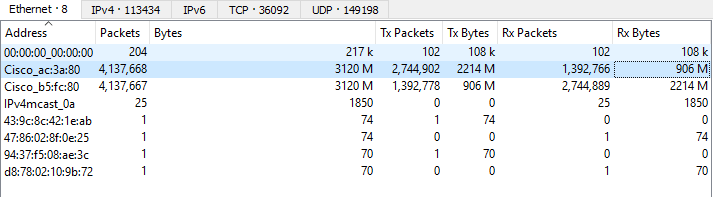
\includegraphics[width = 16cm]{endhost}
		\captionsetup{justification=centering}
		\captionof{figure}{\textit{End Points (Statistics $\rightarrow$ Endpoints)}}
	\end{minipage}
\newline\newline
From the figure above, the main end hosts are \textbf{Cisco\_ac:3a:80} and \textbf{Cisco\_b5:fc:80}. As  there \textbf{few Ethernet end nodes}  with \textbf{many IP end nodes}, we have \textbf{two routers} that sends/receives packets from many remote devices during the entire capture period. For \textbf{Cisco\_ac:3a:80}, the total amount of \textbf{transmitted packets} is \textbf{2,744,902} and the total amount of \textbf{received packets} is \textbf{1,392,766}. The total number of \textbf{transmitted bytes} is \textbf{2214MB} and the total number of \textbf{received bytes} is \textbf{906MB}. \newline
For \textbf{Cisco\_b5:fc:80}, the total amount of \textbf{transmitted packets} is \textbf{1,392,778} and the total amount of \textbf{received packets} is \textbf{2,744,902}. The total number of \textbf{transmitted bytes} is \textbf{906MB} and the total nnumber of \textbf{received bytes} is \textbf{2214MB}. \newline
All transmitted packets \&bytes of \textbf{Cisco\_b5:fc:80} are received by \textbf{Cisco\_b5:fc:80} and vice versa.
\subsection{The number of packet and total bytes of FTP, SSH, DNS,  and HTTP}
In order to identify the total number of packets and bytes trasmitted using File Transfer Protocol (FTP), Secure Shell (SSH), Domain Name System (DNS) and Hypertext Transfer Protocol (HTTP), we have to know the reserved port numbres that are being allocated to these services. The ports allocated for each of these services are as shown in the diagram below:
\begin{figure}[h!]
\centering
	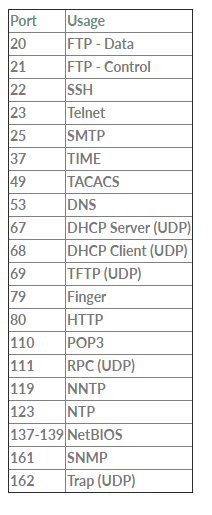
\includegraphics[height = 10cm]{ports}
	\caption{\textit{Well-Known Ports (https://networking.ringofsaturn.com/Protocols/wellknownports.php)}}
\end{figure}

\begin{enumerate}
	\item \textbf{FTP}
	\newline
	The port numbers that are being reserved for FTP is \textbf{20} and \textbf{21}. FTP uses two TCP connections for communication. Port 20 to pass control information and Port 21 to send the data files between the client and the server. The connection has to be established before the files can actually be sent across. As FTP is a TCP connection and thus in order to analyze only the traffic on ports 21 and 22, we apply a display filter to the entire captured traffic \textit{(tcp.port $== 20 || $ tcp.port $== 21$)}\newline
	\begin{minipage}{3in}
	\centering
		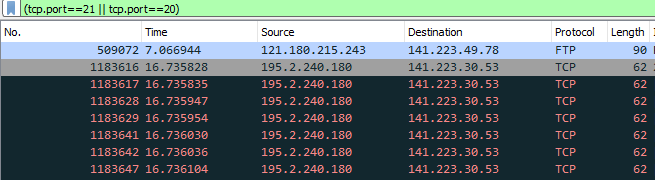
\includegraphics[width = 16cm]{ftpfilter}
		\captionsetup{justification=centering}
		\captionof{figure}{\textit{Filter By FTP Port Numbers}}
	\end{minipage}
	\newline\newline
	\begin{minipage}{5in}
	\centering
		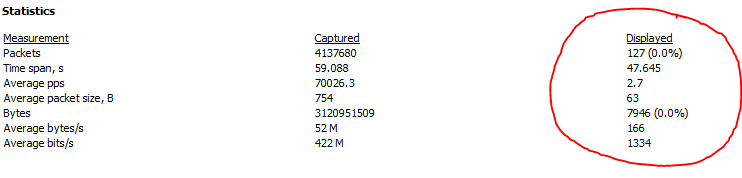
\includegraphics[width = 16cm]{ftppacketsnbytes}
		\captionsetup{justification=centering}
		\captionof{figure}{\textit{FTP Capture Statistics (Stastics $\rightarrow$ Capture File Properties)}}
	\end{minipage}
\newline\newline
	From the capture statistics, we can tell that the total number of packets being captured for FTP is \textbf{127} and the total number of Bytes being captured is \textbf{7946}. FTP takes up close to \textbf{0\%} of the entire network traffic.  From Figure 4, we can tell that there are two Source Destination, \textbf{121.180.215 and 195.2.240.180} and two destination addresses, \textbf{141.223.49.78 and 141.223.30.53}.This sequence of captured traffic is probably the exchange of files (63.568kb) between POSTECH webpages and a client's computer as the IP prefix for POSTECH is \textit{141.223.xx.xx}.
	\item \textbf{SSH}
	\newline
	The port number that is being reserved for SSH is \textbf{22}. As SSH is a TCP connection and thus in order to analyze only the traffic on port 22, we apply a display filter to the 		entire captured traffic \textit{(tcp.port $== 22$)}\newline
	\begin{minipage}{3in}
	\centering
		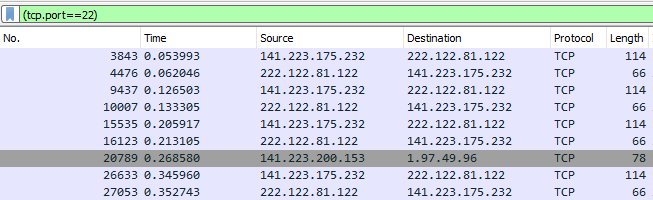
\includegraphics[width = 16cm]{sshfilter}
		\captionsetup{justification=centering}
		\captionof{figure}{\textit{Filter By SSH Port Numbers}}
	\end{minipage}
	\newline\newline
	\begin{minipage}{5in}
	\centering
		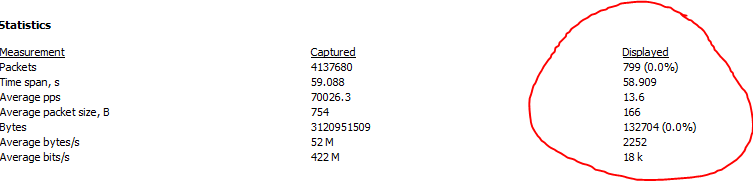
\includegraphics[width = 16cm]{sshpacketsnbytes}
		\captionsetup{justification=centering}
		\captionof{figure}{\textit{SSH Capture Statistics (Statistics $\rightarrow$ Capture File Properties)}}
	\end{minipage}
	\newline\newline
	From the capture statistics, we can tell that the total number of packets being captured for SSH is \textbf{799} and the total number of Bytes being captured is \textbf{132704}. SSH takes up close to \textbf{0\%} of the entire network traffic. SSH is typically used to log into a remote machine and execute commands and can be used to transfer files using the associated SSH file transfer (SFTP) or secure copy protocols (SCP). SSH uses the client-server model.\newline\newline
\begin{minipage}{5in}
	\centering
		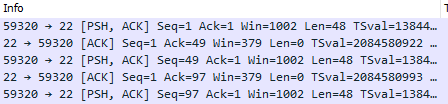
\includegraphics[width = 16cm]{pshack}
		\captionsetup{justification=centering}
		\captionof{figure}{\textit{SSH Traffic Info}}
	\end{minipage}
	\newline\newline
From Figure 9, the [ACK] indicates that a host is acknowledging having received some data, and the [PSH,ACK] indicates the host is acknowledging receipt of some previous data and also transmitting some more data. This sequence of captured data is thus probably the transfers of files between a Postech Server (Identifiable by IP Address Prefix) and a Client's Computer.
	\item \textbf{DNS}
	\newline
 	 A DNS server listens for requests on port \textbf{53 (both UDP and TCP)}. In order to analyze both TCP and UDP traffic on port 53, we apply a display filter to the entire captured traffic \textit{(tcp.port $== 53$ $||$ udp.port $== 53$)}\newline
	\begin{minipage}{3in}
	\centering
		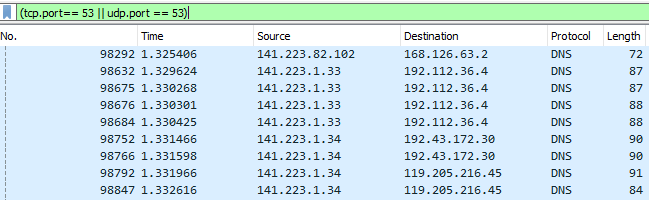
\includegraphics[width = 16cm]{dnsfilter}
		\captionsetup{justification=centering}
		\captionof{figure}{\textit{Filter By DNS Port Numbers}}
	\end{minipage}
	\newline\newline
	\begin{minipage}{5in}
	\centering
		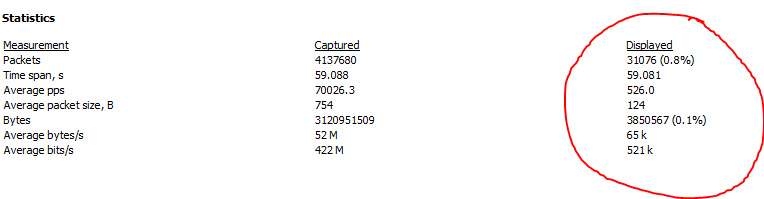
\includegraphics[width = 16cm]{dnspacketsnbytes}
		\captionsetup{justification=centering}
		\captionof{figure}{\textit{DNS Capture Statistics (Statistics $\rightarrow$ Capture File Properties)}}
	\end{minipage}
	\newline\newline
From the capture statistics, we can tell that the total number of packets being captured for DNS is \textbf{31076} and the total number of Bytes being captured is \textbf{3850567}. DNS takes up about \textbf{0.8\%} of the entire network traffic.\newline
\begin{minipage}{5in}
	\centering
		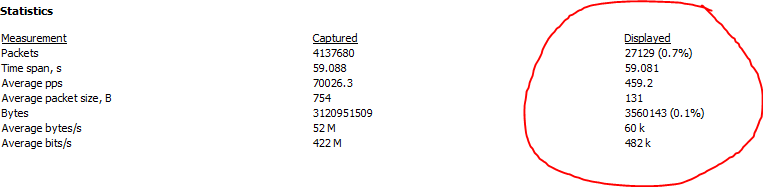
\includegraphics[width = 16cm]{udpdns}
		\captionsetup{justification=centering}
		\captionof{figure}{\textit{DNS (UDP) Capture Statistics}}
		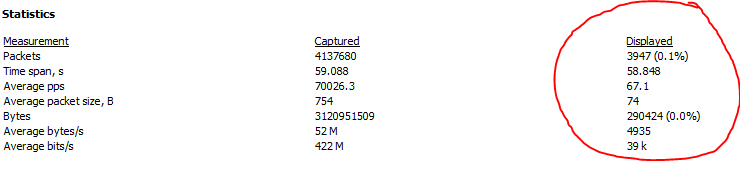
\includegraphics[width = 16cm]{tcpdns}
		\captionsetup{justification=centering}
		\captionof{figure}{\textit{DNS (TCP) Capture Statistics}}
	\end{minipage}
	\newline\newline
DNS realizes UDP as its main transport layer protocol as it is much faster than TCP, which requires a 3 way handshake. TCP is generally used for transmitted large amount of information ($>$ 512 bytes). Comparing Figure 12 and 13, this is true for the captured network traffic as \textbf{more UDP pfacknets (27129)} are being sent over the network as compared to TCP packets (3947).
	\item \textbf{HTTP}
	\newline
	The port number that is being reserved for HTTP is \textbf{80}.As HTML is a TCP connection and thus in order to analyze only the traffic on port 80, we apply a display filter to the 		entire captured traffic \textit{(tcp.port $== 80$)}\newline
	\begin{minipage}{3in}
	\centering
		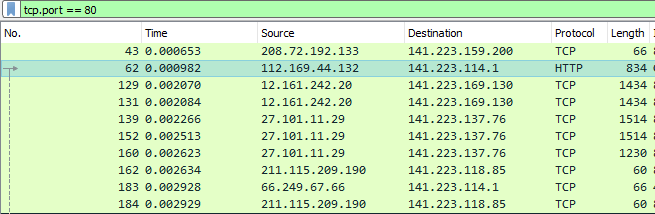
\includegraphics[width = 16cm]{httpfilter}
		\captionsetup{justification=centering}
		\captionof{figure}{\textit{Filter By HTTP Port Numbers}}
	\end{minipage}
	\newline\newline
	\begin{minipage}{5in}
	\centering
		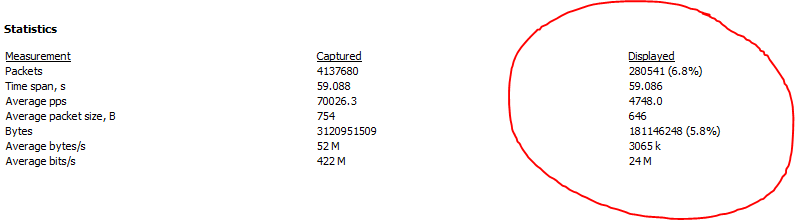
\includegraphics[width = 16cm]{httppacketsnbytes}
		\captionsetup{justification=centering}
		\captionof{figure}{\textit{HTTP Capture Statistics (Statistics $\rightarrow$ Capture File Properties)}}
	\end{minipage}
	\newline\newline
	HTTP is used by the World Wide Web and it defines how messages are formatted and transmitted by browser. As such, we expect HTTP requests to take up a rather significant portion of the captured traffic. From the capture statistics, we can tell that the total number of packets being captured for HTTP is \textbf{280541} and the total number of Bytes being captured is \textbf{181146248}. HHTP takes up close to \textbf{8\%} of the entire network traffic. From Figure 14, we can tell that most of the HTTP traffic are actually between POSTECH's webpages (Identifiable by the IP prefix) and a client's computer. \newline
\end{enumerate}
\subsection{Select  two  applications  other  than  the  aforementioned  applications,  and  print  out  the  number  of packets and the bytes of the traffic which allocates well-known  port  number  (TCP/UDP 1 - 1024) }
The two other applications that I have selected are \textbf{DHCP (Dynamic Host Configuration Protocol)} and \textbf{SMTP (Simple Mail Transfer Protocol)}.

\begin{enumerate}
	\item \textbf{DHCP}
	\newline
	The port numbers that are being reserved for DHCP are \textbf{67} and \textbf{68}. DHCP uses two UDP connections for communication., port 67 for the server and port 68 for the client. The interaction between DHCP clients and servers enables a client to obtain its IP address and corresponding configuration information from a DHCP server. As DHCP utilises a UDP connection, in order to analyze only the traffic on ports 67 and 68, we apply a display filter to the entire captured traffic \textit{(udp.port $== 67 || $ udp.port $== 68$)}\newline
	\begin{minipage}{3in}
	\centering
		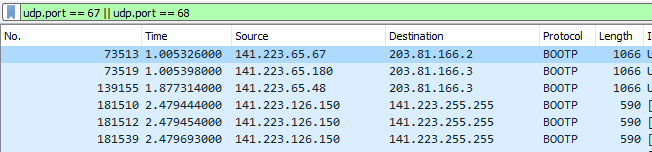
\includegraphics[width = 16cm]{udpfilter}
		\captionsetup{justification=centering}
		\captionof{figure}{\textit{Filter By DHCP Port Numbers}}
	\end{minipage}
	\newline\newline
	\begin{minipage}{5in}
	\centering
		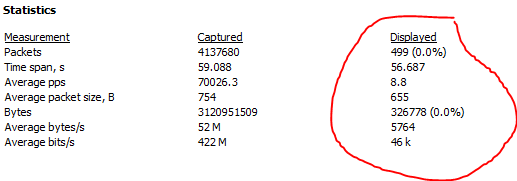
\includegraphics[width = 16cm]{dhcpstatistics}
		\captionsetup{justification=centering}
		\captionof{figure}{\textit{DHCP Capture Statistics (Stastics $\rightarrow$ Capture File Properties)}}
	\end{minipage}
\newline\newline
	From the capture statistics, we can tell that the total number of packets being captured for DHCP is \textbf{499} and the total number of Bytes being captured is \textbf{326778}. DHCP takes up close to \textbf{0\%} of the entire network traffic. The average bytes of each packet being transmitted is about 655. 
	\item \textbf{SMTP}
	\newline
	The port number that is being reserved for SMTP is \textbf{25}. As SMTP utilises both UDP and TCP Connections and thus in order to analyze only the traffic on port 25, we apply a display filter to the entire captured traffic \textit{(tcp.port $== 25$ || udp.port $== 25$)}\newline
	\begin{minipage}{3in}
	\centering
		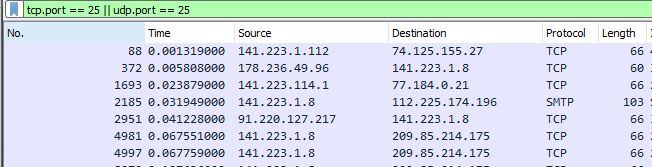
\includegraphics[width = 16cm]{smtpfilter}
		\captionsetup{justification=centering}
		\captionof{figure}{\textit{Filter By SMTP Port Numbers}}
	\end{minipage}
	\newline\newline
	\begin{minipage}{5in}
	\centering
		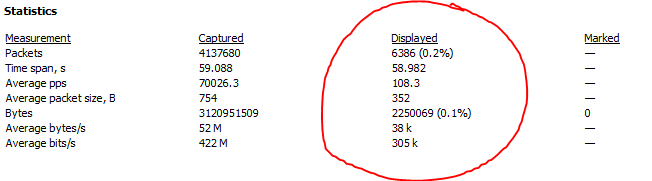
\includegraphics[width = 16cm]{smtpcapturestats}
		\captionsetup{justification=centering}
		\captionof{figure}{\textit{SMTP Capture Statistics (Statistics $\rightarrow$ Capture File Properties)}}
	\end{minipage}
	\newline\newline
	From the capture statistics above, we can tell that the total number of packets being captured for SMTP is \textbf{6386} and the total number of Bytes being captured is \textbf{2250069}. SMTP takes up close to \textbf{0\%} of the entire network traffic. SMTP is generally used for for \textbf{sending e-mail messages between servers \textit{(POSTECH and several other clients for these capture traffic)}} \newline\newline
\begin{minipage}{5in}
	\centering
		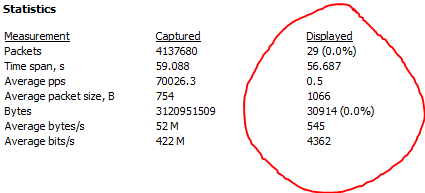
\includegraphics[width = 11cm]{udpsmtp}
		\captionsetup{justification=centering}
		\captionof{figure}{\textit{SMTP (UDP) Capture Statistics}}
		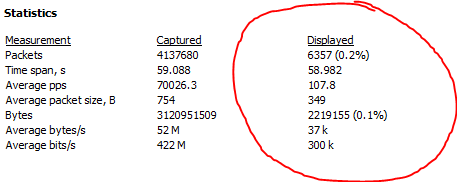
\includegraphics[width = 11cm]{tcpsmtp}
		\captionsetup{justification=centering}
		\captionof{figure}{\textit{SMTP (TCP) Capture Statistics}}
	\end{minipage}
	\newline\newline
Although SMTP realises both TCP and UDP, it makes more sense to use TCP over UDP. SMTP is a mail transport protocol, and in mail every single packet is important. If you lose several packets in the middle of the message the recipient might not even receive the message and if they do they might be missing key information. This makes TCP more appropriate because it ensures that every packet is delivered. Comparing Figure 20 and 21. this is true for the capture network traffic as \textbf{TCP Packets (6357) and bytes (2219155)} are being sent over the network as compared to \textbf{UDP Packets (29) and bytes (30914)}
\end{enumerate}
\pagebreak
\subsection{Enumerate the average packet size, average packet inter-arrival time }
\begin{enumerate}
	\item \textbf{Average Packet Size}
	\newline\newline
	\begin{minipage}{5in}
	\centering
		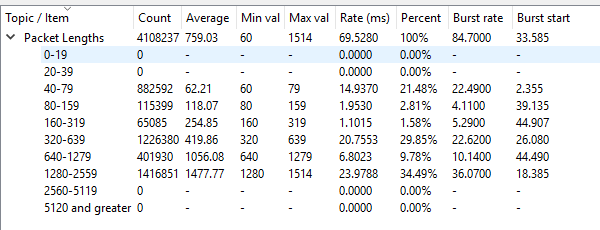
\includegraphics[width = 16cm]{avgpacketsize}
		\captionsetup{justification=centering}
		\captionof{figure}{\textit{Average Packet Size (Statistics $\rightarrow$ Packet Lengths)}}
	\end{minipage}
	\newline\newline
	There were \textbf{4108237 packets} comprising roughly \textbf{3120.95MB} of traffic throughout the capture period. The \textbf{average packet size} for the these packets is \textbf{759.03 bytes}. Majority of the packets are between 1280 - 2559 bytes, and we can tell that higher the amount of byte being trasferred, the higher the transfer rate\textit{(ms)} will be.
	\newline\newline
	\item \textbf{Average Packet Inter-arrival Time}
	\newline\newline
	\begin{minipage}{5in}
	\centering
		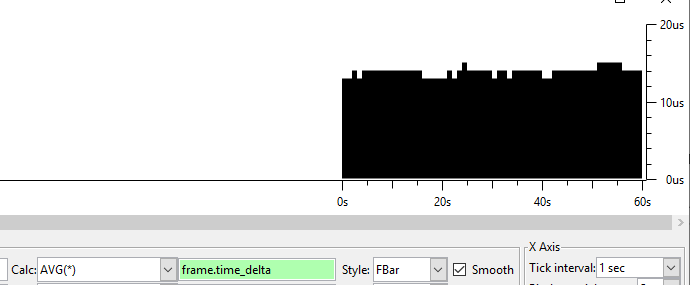
\includegraphics[width = 16cm]{interarrivaltime}
		\captionsetup{justification=centering}
		\captionof{figure}{\textit{Average Packet Inter-Arrival Time (Statistics $\rightarrow$ I/O Graph)}}
	\end{minipage}
	\newline\newline
	From the figure above, we can tell that over the capture period of 60s, the average packet inter-arrival time is somewhere between \textbf{13 to 14$\mu$s} 
\end{enumerate}

\end{document}